\begin{frame}{改めて6面体要素の切り方について復習}
 \begin{table}[hbtp]
    \caption{6面体要素の切り方の例}
    \vspace{-5mm}
    \begin{NiceTabular}{|r|c|c|c|} % 表は項目名を右寄せ、データを中寄せ
       \hline
       名称       &  TransFinite法 & 押し出し法 &  スクリプト法 \\
       \midrule
       概要   & \begin{tabular}{c}形状をレンガ状に分割\\それぞれ構造格子\\を作る(曲面可)\end{tabular}
              & \begin{tabular}{c}平面メッシュを\\特定の方向に\\押し出す\end{tabular}
	      & \begin{tabular}{c}スクリプトで\\作成\\(特殊用途向け)\end{tabular} \\
       \hline
       概念図 & 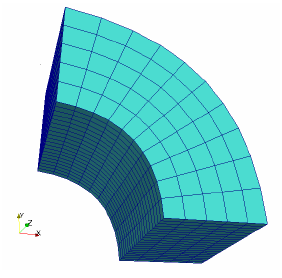
\includegraphics[keepaspectratio,height=15mm]{images/MappedCylinder.png}
              & 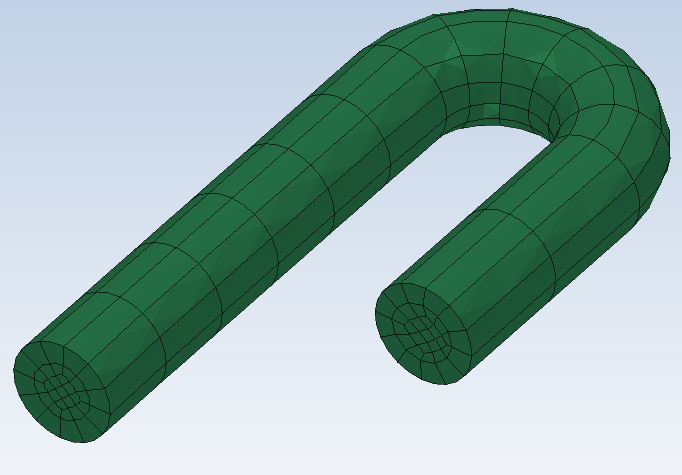
\includegraphics[keepaspectratio,height=15mm]{images/sweep.png}
              & 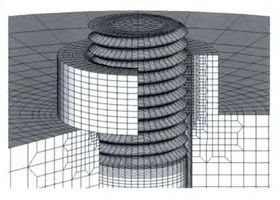
\includegraphics[keepaspectratio,height=15mm]{images/screw.png} \\
       \hline
       参考   & Wikipedia\cite{wiki}
	      & PrePoMax掲示板\cite{PrePoMax-news}
	      & ネジ解析の教科書\cite{fukuoka}\\
       \hline
       注意点 & \begin{tabular}{c}マルチブロック必須\\隣接ブロックと面を\\共有していないと割れ\end{tabular}
	      & 隣接との整合難
	      & アルゴリズム作成難 \\
       \hline
    \end{NiceTabular}
  \end{table}
\end{frame}
